\subsection{Dataset Processing and Model-Ready Representation}

After the COMSOL simulation results were exported, the raw numerical files were converted into a unified machine-learning dataset. This stage was required because the exported COMSOL tables are solver-oriented: they store physical fields in wide CSV format, include metadata rows, and separate temperature, displacement, stress, strain, material parameters, and mesh information into different files. In contrast, the neural models considered in this work require a consistent numerical representation with aligned spatial points, synchronized time steps, normalized physical channels, and clearly separated dynamic and static information.

The purpose of the preprocessing stage was therefore not to prepare data for only one architecture. Instead, the same processed representation was used as a common source for several surrogate-model families. Graph-based models can use the mesh connectivity and edge attributes, operator-learning models can use the spatio-temporal field tensor, and coordinate-based models can sample points in space and time. This reduces duplication and ensures that model comparison is based on the same physical data rather than on different preprocessing assumptions.

The raw dataset was stored in the directory
\[
\texttt{datasets/<dataset\_id>/raw/}.
\]
A typical COMSOL export consisted of several CSV files:
\[
\texttt{data\_temperature.csv},\quad
\texttt{data\_displacement.csv},\quad
\texttt{data\_strain.csv},
\]
\[
\texttt{data\_stress\_1.csv},\quad
\texttt{data\_stress\_2.csv},\quad
\texttt{data\_stress\_3.csv},\quad
\texttt{data\_materials.csv}.
\]
The mesh was exported separately as a COMSOL text mesh file with the extension \(\texttt{.mphtxt}\). Scenario-level information, such as the simulated material and source configuration, was stored in a separate configuration file.

\begin{figure}[H]
    \centering
    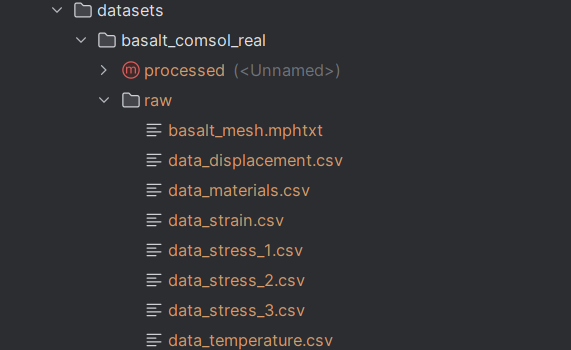
\includegraphics[width=0.95\textwidth]{chapters/chapter4/raw_dataset_folder.png}
    \caption{Folder with all initial raw files of dataset.}
    \label{fig:raw_comsol_csv_header}
\end{figure}

Each CSV file contains COMSOL metadata rows and a numerical table. Metadata rows begin with the symbol \(\texttt{\%}\) and describe the model, version, date, dimensionality, number of nodes, and exported expressions. The actual data table begins from the row containing the coordinate columns. In the exported files, spatial coordinates are represented by
\[
X,\quad Y,\quad Z.
\]
The remaining columns contain physical fields written in the COMSOL format

\begin{figure}[H]
    \centering
    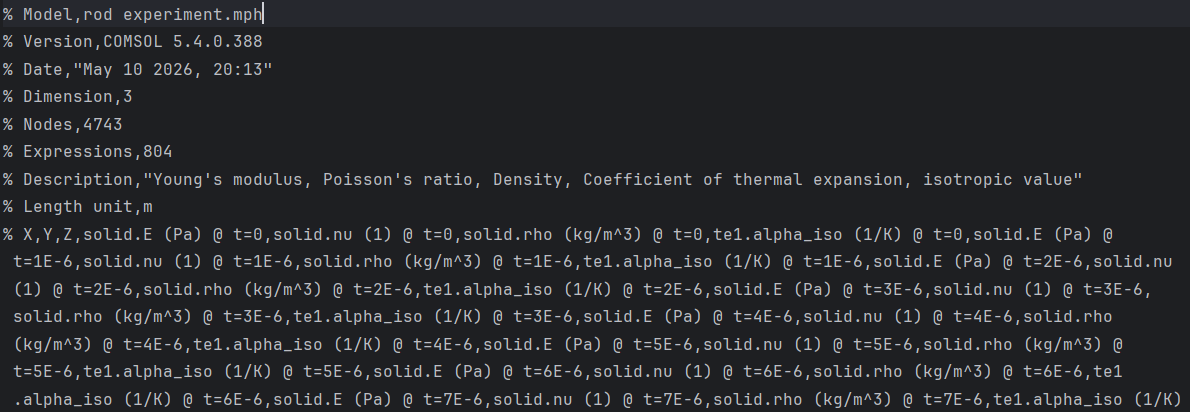
\includegraphics[width=0.95\textwidth]{chapters/chapter4/example_of_dataset.png}
    \caption{Example of a raw COMSOL CSV export.}
    \label{fig:raw_comsol_csv_header}
\end{figure}

This naming convention allows the preprocessing script to extract three pieces of information from each column: the physical variable, its unit of measurement, and the simulation time.

During CSV cleaning, service rows were skipped, the real header row was detected, and only supported physical exports were parsed. Non-numerical entries were converted where possible, while invalid or missing values were handled before tensor construction. This was necessary because the exported variables have different physical meanings and numerical scales: temperature is measured in kelvin, displacement in meters, stress in pascals, strain is dimensionless, and material parameters may have much larger magnitudes.

A separate coordinate-alignment step was required because different COMSOL exports may contain different point sets or the same points in a different order. Therefore, the files cannot be merged reliably by row index. A reference coordinate array was selected, and the remaining fields were mapped to this reference using nearest-neighbor matching in coordinate space:
\[
j(i) =
\arg\min_j
\left\|
\mathbf{r}^{\mathrm{ref}}_i -
\mathbf{r}^{\mathrm{src}}_j
\right\|_2 .
\]
Here, \(\mathbf{r}^{\mathrm{ref}}_i\) is the \(i\)-th coordinate in the reference node set, and \(\mathbf{r}^{\mathrm{src}}_j\) is a coordinate from another exported file. This step produced a single aligned node set shared by all physical fields.

After alignment, the data were separated into dynamic and static features. Dynamic features describe the time-dependent state of the thermoelastic process. These include temperature, displacement components, velocity components, stress components, and strain components. Static features describe quantities that do not change during one simulation, such as spatial coordinates, material parameters, source-region indicators, distance to the source, and scenario-level parameters. Material properties are not treated as prediction targets; they are used as conditioning information for the models.

The dynamic part of the dataset was assembled into a spatio-temporal tensor
\[
\mathbf{S} \in \mathbb{R}^{N_t \times N_p \times F_d},
\]
where \(N_t\) is the number of time steps, \(N_p\) is the number of spatial points or mesh nodes, and \(F_d\) is the number of dynamic physical channels. For one time step \(n\), the state of the simulated medium is represented as
\[
\mathbf{S}_n \in \mathbb{R}^{N_p \times F_d}.
\]
The static part was stored as
\[
\mathbf{A} \in \mathbb{R}^{N_p \times F_s},
\]
where \(F_s\) is the number of static node or scenario features.

Normalization was applied separately to dynamic and static features. For each feature channel, the mean and standard deviation were computed and saved for later denormalization. The normalized value was calculated as
\[
\widetilde{x}
=
\frac{x-\mu}{\sigma+\varepsilon},
\]
where \(x\) is the original feature value, \(\mu\) is the mean value of the corresponding channel, \(\sigma\) is its standard deviation, and \(\varepsilon\) is a small constant used for numerical stability. Separate normalization statistics are important because dynamic physical fields and static material parameters have different distributions and units.

For graph-based models, the aligned coordinates were additionally converted into a graph representation. If the exported \(\texttt{.mphtxt}\) file was available and compatible with the aligned node set, mesh connectivity was used to construct graph edges. If the mesh connectivity could not be used, a nearest-neighbor graph was constructed from the node coordinates. For an edge from node \(i\) to node \(j\), the edge attribute vector was defined as
\[
\mathbf{e}_{ij}
=
\left[
x_j-x_i,\,
y_j-y_i,\,
z_j-z_i,\,
\left\|
\mathbf{r}_j-\mathbf{r}_i
\right\|_2
\right].
\]
The first three components describe the relative spatial offset between neighboring nodes, while the last component stores the Euclidean distance.

Training pairs were generated from the processed time sequence. Depending on the model type, the processed dataset can be used either as full-field states, coordinate-time samples, temporal sequences, or graph trajectories. For one-step transition learning, the target can be represented as the state increment
\[
\Delta \mathbf{S}_n
=
\mathbf{S}_{n+1}
-
\mathbf{S}_n .
\]
This delta representation is useful for transient dynamics because the model learns the local change of the physical state between consecutive time steps rather than predicting the complete field independently at every step.

The output of the preprocessing stage was a set of processed artifacts stored in
\[
\texttt{datasets/<dataset\_id>/processed/}.
\]

\begin{figure}[H]
    \centering
    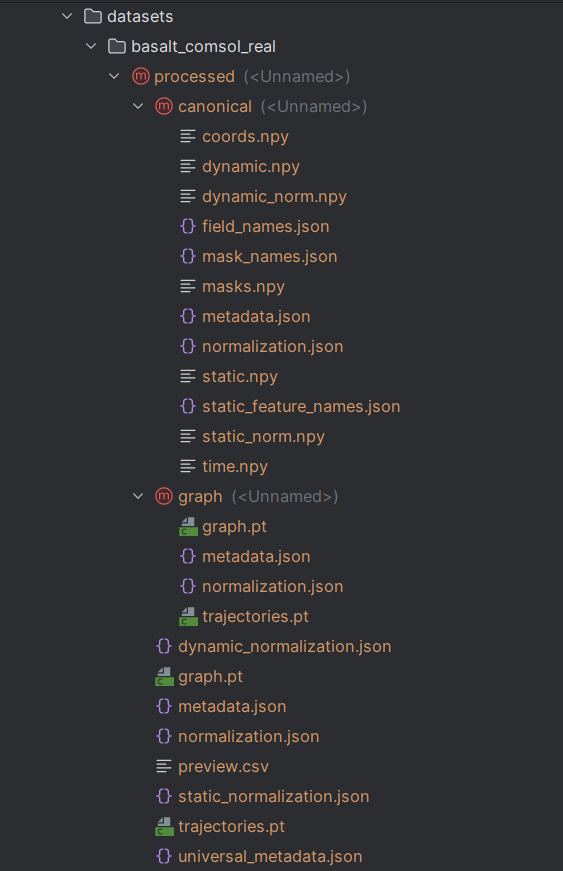
\includegraphics[width=0.95\textwidth]{chapters/chapter4/processed_dataset_folder.png}
    \caption{Folder including all processed from dataset files.}
    \label{fig:raw_comsol_csv_header}
\end{figure}

The most important artifacts are summarized in Table~\ref{tab:processed_dataset_artifacts}.

\begin{table}[H]
\centering
\caption{Processed dataset artifacts produced from COMSOL exports.}
\label{tab:processed_dataset_artifacts}
\begin{tabular}{p{0.32\textwidth} p{0.58\textwidth}}
\hline
\textbf{Artifact} & \textbf{Purpose} \\
\hline
\texttt{coords.npy} &
Aligned spatial coordinates of the computational points or mesh nodes. \\
\hline
\texttt{dynamic.npy} &
Time-dependent physical fields stored as a spatio-temporal tensor. \\
\hline
\texttt{static.npy} &
Static node, material, and scenario features. \\
\hline
\texttt{time.npy} &
Simulation time values corresponding to the dynamic states. \\
\hline
\texttt{normalization.json} &
Normalization statistics required for scaling and denormalization. \\
\hline
\texttt{metadata.json} &
Dataset metadata, including feature names, dimensions, time-step information, and processing configuration. \\
\hline
\texttt{graph.pt} &
Graph representation used by graph-based models: edge index, edge attributes, coordinates, and static node features. \\
\hline
\texttt{trajectories.pt} &
Prepared transition samples or trajectory fragments for models that learn temporal state evolution. \\
\hline
\texttt{preview.csv} &
Diagnostic summary used to inspect feature ranges and verify the correctness of preprocessing. \\
\hline
\end{tabular}
\end{table}

The complete transformation pipeline can be summarized as
\[
\text{Raw COMSOL exports}
\rightarrow
\text{CSV cleaning}
\rightarrow
\text{coordinate alignment}
\rightarrow
\text{feature separation}
\rightarrow
\text{tensor construction}
\rightarrow
\text{normalization}
\rightarrow
\text{model-ready artifacts}.
\]
For graph-based models, an additional branch is applied:
\[
\text{aligned coordinates}
\rightarrow
\text{mesh or nearest-neighbor connectivity}
\rightarrow
\text{graph representation}.
\]

Thus, the preprocessing stage converts heterogeneous COMSOL outputs into a common numerical dataset that can be reused by different neural surrogate models. This design is important for fair comparison: the models differ in architecture and input representation, but they are trained and evaluated from the same cleaned, aligned, and normalized thermoelastic simulation data.